\section{Sensor systems in smart environments}
In the most general definition a sensor is a device that transforms a physical property into an observable signal. This definition includes traditional systems such as mercury-based thermometers or hair-based hygrometers. Yet nowadays we are usually considering digital sensors that transfer the measured property to a binary signal that can be further processed by computing devices. 
A common variety is the smart sensor that provides additional functionality beyond generating a correct sensing signal \cite{frank2013understanding}. The main goal is to simplify installation and maintenance of distributed sensing systems by having processing close to the measurement device. Early considerations in this domain were put to the standard family IEEE 1451 - IEEE Standard for a Smart Transducer Interface for Sensors and Actuators between 1997 and 2007 \cite{ieee1451}. An additional concept is the Virtual Sensor that includes digital signal processing and conditioning and therefor abstracts the processing steps from devices interfacing the sensor. 
The number of available sensors is very high, but it is possible to restrict them based on application domain. Lewis and Cook et al. \cite{lewis2004wireless,cook2007smart} have proposed a collection for smart environments focused on wireless sensor networks. The overview is shown in table \ref{tab:sen_smart_env}.
\begin{table}[htbp]
  \centering
  \caption{Sensors for smart environments \cite{cook2007smart}}
    \begin{tabular}{rr}
    \toprule
    \textbf{Properties } & \textbf{Measurand} \\
    \midrule
    Physical properties  & Pressure, temperature, humidity, flow \\ \addlinespace
    Motion properties  & Position, velocity, angular velocity, acceleration \\ \addlinespace
    Contact properties  & Strain, force, torque, slip, vibration \\ \addlinespace
    Presence  & Tactile/contact, proximity, distance/range, motion \\ \addlinespace
    Biochemical  & Biochemical agents \\ \addlinespace
    Identification  & Personal features, RFID or personal ID \\
    \bottomrule
    \end{tabular}%

  \label{tab:sen_smart_env}%
\end{table}%
This sensor categorization is based on the property to be measured and is agnostic to the specific measurement technology. Physical properties, such as pressure, temperature, humidity and flow, can also be noted as environmental properties. They are measurements that determine the state of the smart environment, e.g. temperature in different rooms, or the current water usage. Motion properties denote the movement parameters of actors in this environment and can refer to both humans and machines. Angular velocity is important in self-localization of robots in an environment. Contact properties groups the different types of interaction between surfaces in the smart environment and actors. Presence as a group is similar to motion paramteres, but does not require a series of measurements for tracking an actor. Biochemical sensors enable measuring the presence of specifc chemical compounds in the environment and are most suited for measuring pollution or air quality. Finally, identification of actors allows to provide personalized services and can be realized with different methods ranging from tags to biometric systems.

While this listing provides a decent overview of sensing properties in smart environments it is abstracted from sensor technologies. Various types of sensors, including capacitive proximity sensors, allow us to detect multiple of these properties and thus providing a higher flexibility. Therefore it is possible to provide an inverse listing of sensor technologies that allow measuring different properties. A short overview of sensor technologies with this capabilities and that are commonly used in smart environments is given in table \ref{tab:sen_tech_prop}. In the following sections I want to give an overview on how these sensor systems are used in this domain, in order to provide a basis for the benchmarking model that will be introduced in section \ref{ch:benchmark}.
\begin{table}[htbp]
  \centering
  \caption{Sensing technologies and measured properties}
    \begin{tabular}{rr}
    \toprule
    \textbf{Technology} & \textbf{Properties} \\
    \midrule
    RGB cameras  & Motion, Presence, Identification \\ \addlinespace
    Infrared cameras & Motion, Presence, Contact \\ \addlinespace
    Ultrasound sensing & Motion, Presence, Contact, Identification \\ \addlinespace
    Microphone arrays & Motion, Presence, Contact, Identification \\ \addlinespace
    Radiofrequency sensing & Motion, Presence, Identification \\
    \bottomrule
    \end{tabular}%
  \label{tab:sen_tech_prop}%
\end{table}%

\subsection{RGB cameras}
\begin{figure}[h]
\centering
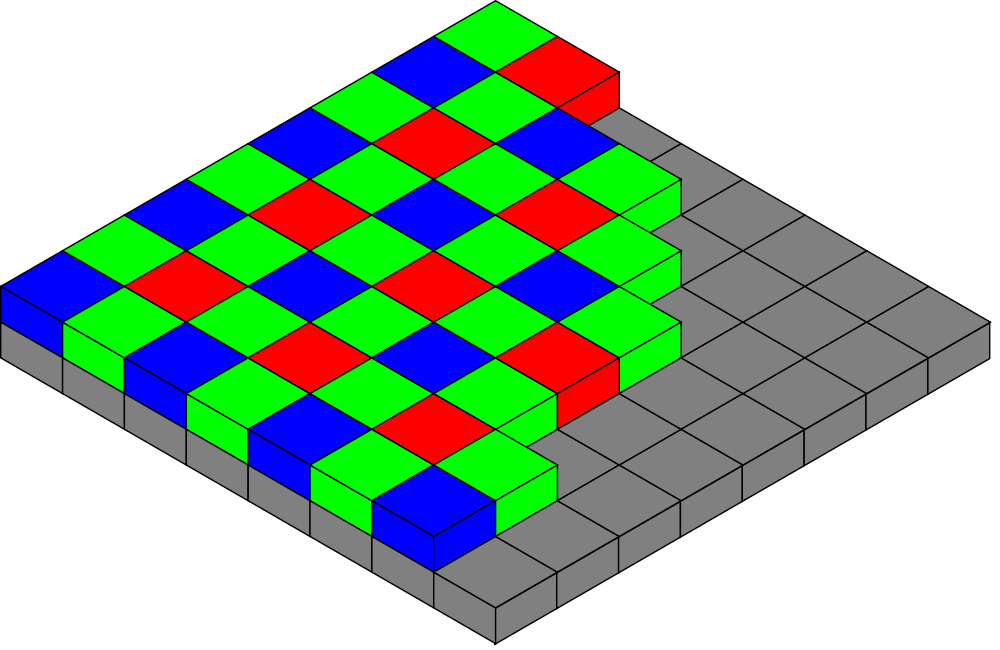
\includegraphics[width=0.4\textwidth]{images/bayer_pattern_on_sensor}
\caption{A bayer pattern on a sensor in isometric perspective \cite{img_bayer_pattern}}
\label{fig:bayer_pattern}
\end{figure}
A RGB camera is an image processing device that processes light in the visible spectrum, similar to the human eye. Modeled after the retina it has three distinct color channels - red, green and blue. There are different methods available to distinguish these channels from visible light, such as Bayer filters (Figure \ref{fig:bayer_pattern}) in front of a single sensor or using multiple sensors behind a prism.
The usage of cameras in smart environments is very common. I will present five different examples and afterwards will specify how they are linked to the properties that were defined previously.
Tabar et al. have been using a combined system of cameras, RF transmitters and wearable sensors in a home care scenario \cite{tabar2006smart}. The cameras are used to improve the accuracy of the accelerometer-based fall detection by eliminating false positives. Once a fall event occurs an algorithm tracks the posture of detected humans in the scene. They used an edge detector to distinguish the human body from other objects and applied a heuristic to differentiate lying and standing.  Additionally a face detector was used to improve the recognition of human objects. Combining this with information from the fall detecting sensor and a RF based localization system they were able to achieve a good reliability in eliminating false positive alerts.
\begin{figure}[h]
\centering
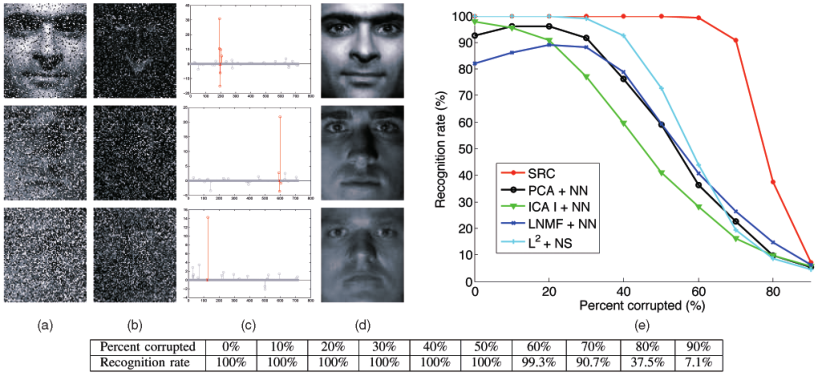
\includegraphics[width=0.9\textwidth]{images/facerec_noise}
\caption{Recognition under random corruption. (a) Top row: 30 percent of pixels are corrupted. Middle row: 50 percent corrupted. Bottom row: 70 percent corrupted. (b) Estimated errors (c) Estimated sparse coefficients (d) Reconstructed images (e) The recognition rate across the entire range of corruption for various algorithms. Newly presented (red curve) significantly outperforms others, performing almost perfectly upto 60 percent random corruption \cite{wright2009robust}}
\label{fig:facerec_noise}
\end{figure}

Pentland and Choudhury provided an overview of vision-based face recognition systems in the domain of smart environments \cite{pentland2000face}. The systems are able to identify users and recognize facial expressions. The proposed applications in smart environments include personalized shopping experiences based on customer recognition, behavior monitoring in child care facilities and emotion-aware systems that react to the user's current awareness. The described techniques include PCA-supported, eigenvector-based classification, face-based localization and systems based on local feature analysis. Newer systems are able to operate well in unconstrained environments, that include varying expression and illumination, ageing of persons, occlusion and disguise \cite{wright2009robust} (example of robustness with regard to image corruption in Figure \ref{fig:facerec_noise}).
\begin{figure}[h]
\centering
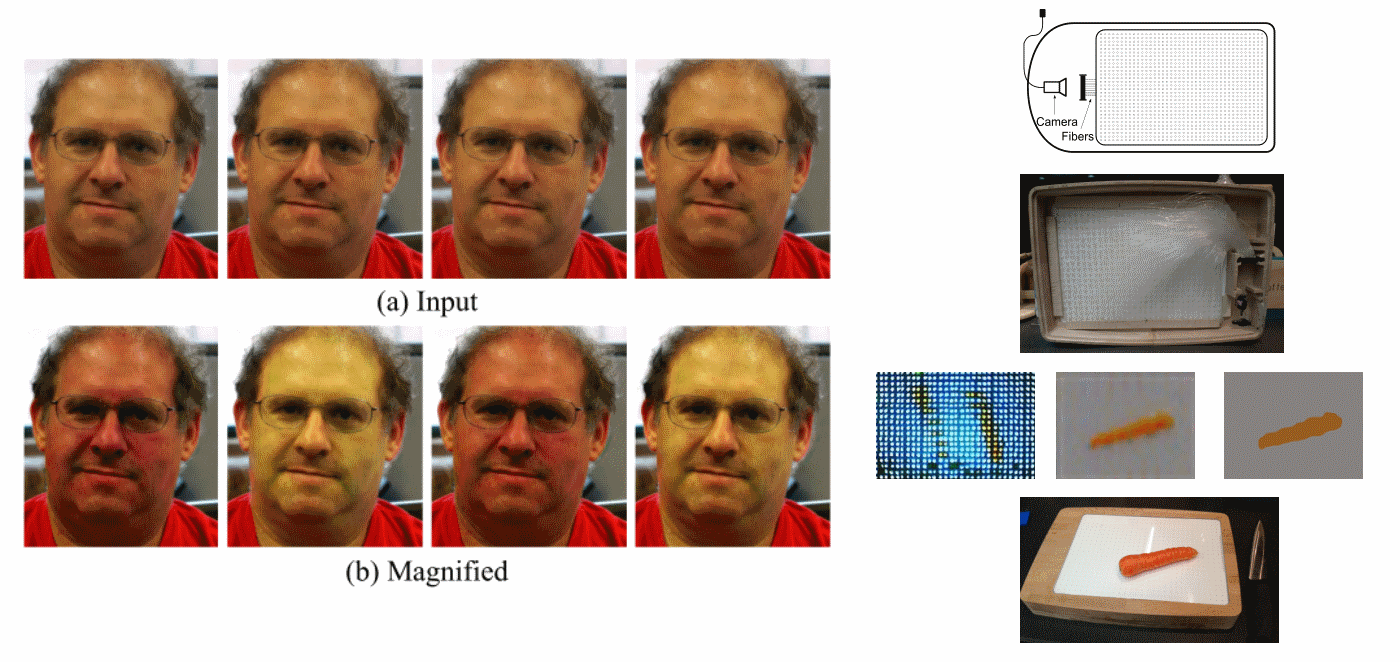
\includegraphics[width=0.7\textwidth]{images/rgb_euler_food}
\caption{\emph{Left}: Eulerian Video Magnification to attenuate the human pulse with original (a) and amplified (b) video sequence  \cite{Wu2012}. \emph{Right}: FoodBoard schematics (top), underside view (second row), original, reconstructed and segmented image (third row) and final system (bottom) \cite{pham2013foodboard}}
\label{fig:rgb_euler_food}
\end{figure}

An example for a novel image processing method that is useful in smart environments was presented by Vu et al. in 2012 \cite{Wu2012}. They are using  temporal variances of pixel values to exaggerate spatial movements and color changes that would typically be invisible to the naked eye. The method is called Eulerian Video Magnification and uses a combination of spatial decomposition and temporal filtering applied to adjacent frames. It can be tuned to different time-frequency bands to attenuate different classes of signals. Some of the proposed applications include the tracking of breathing rates of infants by attenuating chest movement, or the tracking of subtle movements, such as vibration in appliances. The example shown in Figure \ref{fig:rgb_euler_food} on the left is using a magnification of colors, in order to identify the heart rate of a person. The latter can be used for personal health applications, e.g. by integrating the system into the bath room mirror to provide an unobtrusive daily measurement and give the user feedback over a longer period of time.

A final example in this section is the FoodBoard, a smart chopping board that uses image processing to recognize the food items that are put on it \cite{pham2013foodboard}. It is shown in Figure \ref{fig:rgb_euler_food} on the right. To enable a thin footprint, ambient light is transferred to a camera using glass fibers. The picture is reconstructed and segmented, allowing to identify different items of food that are placed on it. The classification is based on a combination of Fast-Hessian and color histogram feature extractors. Pham et al. were able to distinguish 12 different ingredients with an accuracy between 59\% and 93\%. The system can be used to support dietary monitoring, give recipe guidance or support visually impaired users in identifying and tracking food.
\subsection{Infrared cameras}
Infrared imaging is using the same sensors that are suitable for visible light imaging. The difference is that they are tuned to collect electromagnetic waves of a lower wavelength that are just outside of the visible spectrum. This allows for distinct applications, such as thermal imaging, as it is possible to detect heat radiation. One of the earliest prototypes in Ubiquitous Computing designed by PARC was the ORL Active Badge, an infrared emitter that was used to identify persons operating in the environment \cite{Weiser1991}. In smart environments the most common application is using infrared cameras in combination with infrared light sources. This allows to illuminate spaces without visible artifacts to the user, thus providing imaging capabilities in dark rooms, or very specific conditions that may be required by a certain application. Another very interesting option is to use a specific projection of patterns into the scene. Analyzing the returning infrared light it is possible to infer the depth of specific pixels of the camera. This variety is called a depth camera. Particularly in the last few years the research in this domain has expanded strongly, sparked by the availability of an affordable depth camera/RGB camera combination - the Kinect by Microsoft \cite{zhang2012microsoft}. On the following pages we will present various examples of how this device can be used in smart environments to enable different applications in interaction and activity tracking.

Sung et al. have presented a system that is tracking activities of daily life based on the movements of a skeleton that is provided by the Kinect API \cite{sung2011human}. This skeleton model is based on a pose reconstruction algorithm developed by Shotton et al. \cite{Shotton2013} and is used in many different Kinect-based applications. The algorithm is using a method called hierarchical maximum entropy Markov model (MEMM). Each activity is considered to be composed of sub-activities. Based on this assumption a two-level graph is generated using dynamic programming. The system was tested with twelve activities performed in an office, a kitchen, a living room, a bathroom and a bedroom. If the person was part of the training set the precision was 84.3\% and 64.2\% for unknown persons. Some example activities of the acquired dataset are shown in Figure .

A novel method to use the Kinect for fast 3D reconstruction of scenes was presented by Izadi et al. in 2011 \cite{Izadi2011}. The basic premise is to use a fast registration method to combine point clouds that are generated by the system and continuously extend and optimize the current model of the scene. They are using a GPU-based ICP implementation to track the position of the camera in six degrees-of-freedom. This allows to reliably integrate the different point clouds into a single voxel grid that can be used to represent and render the scene. They proposed a number of applications ranging from phyiscal simulation of particles in the scene, to system control based on segmenting and tracking the user's hands and their interaction with arbitrary surfaces in the environment. Figure  shows some results of the touch recognition in a reconstructed scene.

Galen has presented a method to use a Kinect in a kitchen to provide touch free interaction \cite{panger2012kinect}. Two different interaction schemes are proposed. The first allows to control the applications with messy hands, the second enables to use other limbs if the hands are currently occupied. Three different test applications have been implemented. A recipe navigator that allows to open and navigate through different recipes. A timer that enables setting different alarm times, similar to a kitchen clock and a music player that can be controlled to choose different stations according to preference. A real life test with five subjects  did also test installation complexity, which was deemed favorable. There were some concerns in clearly distinguishing commands from random movements performed in the kitchen.

The final system based on infrared cameras is an immersive telepresence system developed by Beck et al. \cite{beck2013immersive}. Telepresence enables persons to be present as a representation in a remote place. A typical example is video conferences, but advanced system may include robotics or virtual elements. The presented system is using a single Kinect for each participant. A 3D representation is created based on the depth information of the infrared camera and on-the-fly texturing using the included RGB camera. The virtual user representations are put into a shared virutal environment and can interact with each other. Some variations were tested where local and remote users were decoupled, side-by-side or face-to-face. Different tracing and pointing gestures are supported. The supported applications included the exploration of a virtual city as shown in Figure .

\subsection{Ultrasound sensors}
Ultrasound sensors allow detecting sound wave signals that have a frequency beyond 20kHz and are thus not audible to humans. Their propagation and reflection properties are similar to audible sound waves, thus the generated measurements can be similar. While there are natural sources of ultrasound waves the applications in smart environments do rely on active systems, that combine sound generators and sensors that measure the resulting signal. By timing the time distance between sending the signal and receiving a response it is possible to measure distances between the sender and different object.  If various receivers are used it is possible to localize the sound source, making ultrasound sensing a popular candidate in indoor localization systems. In Figure we can see a sketch of the basic functionality of ultrasound sensing systems on the left, and an example of localization using three receivers and a single source. We will present four different examples on how ultrasound sensors are used in smart environment applications.

The Cricket developed by Pryantha et al. is an example for an indoor localization system based on a badge the tracked object has to wear \cite{priyantha2000cricket}. The badge is periodically sending signals to a set of beacons that determine the distance and calculate a location. Initially it was supposed to solely rely on radiofrequency signals, but was modified to use a combination of RF and ultrasound. The rationale of this decision is the considerably slower speed of sound that simplifies measuring the time-of-flight and thus allows for more precise distance measurements. Consequently this also leads to a better precision in the localization algorithm. Additionally, the system uses some novel methods to deal with interference and multipath issues, that is dealing with reflected signals. As potential applications they propose space-dependent services that are provided as the user is identified in a certain region and guidance scenarios on a floor plan.

\cite{prassler2001robotics}
Describes the robotic wheelchair MAid (Mobility Aid for Elderly and Disabled People). MAid's task is to support and transport people with limited motion skills. It is based on a commercial wheelchair that has been equipped with an intelligent control and navigation system. Conversations with disabled and elderly people and with their physicians indicate that the automatic functions desired in a robotic wheelchair do not include following walls or passing doorways, but do include navigation in narrow, cluttered environments

Watanabe et al. investigate the role of ultrasound sensors in recognizing activities and gestures of a user \cite{watanabe2013ultrasound}. The system is comprised of a microphone attached to a necklace and two speakers that are attached to each wrist. Based on the acquired volume and evaluation of the Doppler effect it is possible to determine both distance of the wrists from the neck and the speed of movement. Watanabe et al. want to determine if this system allows for similar performance compared to other body-worn systems based on accelerometer and gyroscope data. Additionally it was evaluated if external microphones can perform as well as the neck worn microphone. The system was able to recognize 87\% of activities and gestures in a set of 10 test persons if no influencing sound was present. The ultrasound did also improve results if environmental noise was present.

A recent project at the University of Tokyo evaluates the potential of ultrasound in manipulating small particles in free-air \cite{ochiai2013three}. Using standing waves to  create sound pressure notes it is possible to apply a force to small particles that is sufficient to counteract gravity. Using a set of ultrasonic phased arrays it is possible to create these sound pressure nodes at arbitrary positions in three dimensions. Ochiai et al. use this to move small objects around and investigate required object properties and their floating properties. So far the moved items have to be very light and smaller than 2 mm in diameter, resulting in the usage of polystyrene. The technology is also able to hold and move small amounts of fluid. Suggested applications include object manipulation in microgravity environments and projected haptic feedback systems.

\subsection{Microphone arrays}
Microphones are signal receivers that are tuned to detect sound frequency ranges that are audible by humans. Typically they consist of a piezo element that transfers vibration to an electric current that is amplified. A schematic can be seen in Figure . Most human activities produce some kind of sound. As opposed to the presented ultrasound system, microphones typically operate passive. That is there is usually no dedicated signal source, but instead naturally occuring sounds are picked up. By combining microphones or arrays thereof with data processing systems that are aimed at analyzing specifc sound patterns we are able to get feedback on human activities. Looking at smart environments there are numerous use cases that can benefit from microphones as sensors. In this section we will present four different systems that cover a large variety of different applications, ranging from breathing rate detection to estimating the number of speakers in large groups.

Detecting the breathing pattern of a person has several applications in smart environments. Apart from medical applications that require detecting abnormal breathing in risk groups it is also possible to track training progress using such a system or provide a measure for the current attention level in affective computing. Corbishlev et al. investigated using very small microphones in mobile devices to enable detecting the breathing rate \cite{corbishley2008breathing}. The algorithm is designed to be applicable on single ICs, allowing for miniaturization and energy efficiency. Even with the presence of noise the combined score for true negatives and true positives was as high as 91.3\%. Using small and energy efficient systems also enables unobtrusive applications in non-mobile environments, e.g. placing such a system close to the bed to detect the breathing rate while the user is sleeping.

Collaborative applications are an important aspect of smart environments, e.g. to link together meeting places at different places, similar to the presented telepresence applications. If a multitude of speakers is present it gets increasingly difficult to provide a system that enables proper speech transmission for all participants. Using an array of microphones it is possible to focus the attention on the person currently speaking and filter out environmental noise. A project at Microsoft Research investigated using a maximum likelihood of two known techniques, beamforming and speech source localization, to enable a reliable speaker selection \cite{zhang2008maximum}. Additionally the framework enables a good adaptation even if directional microphones are used that are placed close to each other. The method provides a real life accuracy of more than 90\%.

A fairly new work was performed by Xu et al. \cite{xu2013crowd++}, called Crowd++. Their idea is to use smartphone microphones to identify the number of speakers in crowded environments. Such system could be used to estimate the number of persons in a given place and potentially react quickly if a crowd panic may occur. The method is based on an unsupervised machine learning classification of short audio parts that are picked up by the individual microphones in the handsets. It was tested by 120 participants in 10 different environments and allowed detecting the number of persons with an average error of 1.5 persons. No dedicated hardware is required to achieve this precision, enabling an application using off-the-shelf smartphones.

Microphones can also be used to analyse the mechanical surface waves that occur when objects interact with each other. Harrison et al. have designed TapSense, a microphone based sensor system that improves touch interaction by classifying the sounds created by different objects hitting the surface \cite{harrison2011tapsense}. In particular different parts of the hand can be distinguished, including nail, knuckle or tip. Potential applications are improving touch interaction on touch screens by enabling different forms of interaction, but also can be adapted to mobile devices, that typically have less interaction space and increase the expressiveness of different touch gestures. The achievable accuracy was between 95\% using four different input types up to 99\% when using just two input sets, such as finger and pen.

\subsection{Radiofrequency sensing}
Radiofrequency sensing is a traditional field for sensors. Radar is a system that uses radio waves to acquire direction, speed, distance or altitude of objects and was developed at the beginning of World War II. This variety is using active sensing and emits radio waves that are reflected by objects. Most applications in smart environments similarly rely on active systems. A popular signal source are WiFi signals, intended to wirelessly transmit information between several systems. The systems are wide-spread, with all smartphones possesing two or more wireless technologies (typically 4G/3G/GSM for long range communication, WLAN for medium range communication and Bluetooth/NFC for short range communication) that can be used in coordination with stations placed in the environment. The signal processing of the wireless LAN sets generates some additional data that can be used, most notably the signal strength (RSSI). We will present different systems that show some different ways how radiofrequency sensing can be used in smart environments.

Radiofrequency based systems are very popular for indoor localization applications. We previously glimpsed at the difficulty of time-of-flight systems in the electromagnetic specturm. Thus most systems rely on a different approach, using the received signal strength (RSSI). If the initial signal strength is known and we have a good estimate how the signal propagates we can estimate the loss of signal strength at a certain distance. An accepted work that helped shaping this domain is the system created by Sugano et al. in 2006 that uses a ZigBee-based network with a limited number of nodes receiving RSSI information \cite{sugano2006indoor}. Based on this it is possible to locate one or more users with an error between 1.5-2m. This often is sufficient to distinguish the room a person is currently in, enabling a room-based system adaptation, which is suitable for many applications.

A different approach for RSSI based systems was presented by Wilson and Patwari in 2010 \cite{wilson2010radio}. They are using tomography methods to determine the location of users. By placing a large number of sensors on the outer limits of the environment and creating a unique link between each, it is possible to infer the position based on the signal attenuation when a person moves in the environment. The human body absorbs some of the signal, resulting in a reduced received RSSI in the affected nodes. The error for standing persons was between 0.64cm for a single person and 1.10cm for two persons. An image of the test area is shown in Figure on the right.

A final system that provides a localization is WiTrack, presented by Adib et al in 2013 \cite{adib20133d}. It uses the signal reflected by the human body to provide a location estimate based on time-of-flight. As mentioned previously this is challenging due to the propagation speed within the electromagnetic field. To overcome this issue they are using a method called frequency modulated carrier wave that transfers time differences to the frequency domain. Looking at the spectrum of received signal these shifts can be analyzed. The resulting location has an accuracy of 10-13 cm in x and y and 21 cm in z dimension. Additional use cases are provided in determining coarse arm or foot gestures and enabling an accurate detection of falls of a person. Some limitations of this approach include a restriction to just one person and that the tracked object has to move.

The final radiofrequency system I want to present is WiSee, developed at the University of Washington by Pu et al. \cite{pu2013whole}. They are using Wi-Fi to enable gesture recognition in large areas without requiring a line-of-sight. They are analyzing the Doppler shift resulting from human activity in order to classify different gestures. They are using MIMO (multiple input multiple output) to distinguish between non-interacting persons in the environment and the person performing gestures. To equip a whole appartment only a single receiver and two transmitters are necessary. The achievable accuracy varies according to persons present and number/type of devices involved but peaks at an accuracy of 94\% for detecting nine different whole body gestures. The supported gestures and their Doppler profiles are shown in Figure .